% Document class report-template accepts either: project-plan or final-report option
\documentclass[project-plan]{report-template}

% Packages I want to use in my report.
\usepackage{graphicx}
\usepackage{amsmath}
\usepackage{blindtext}

% Directory where I save my figures.
\graphicspath{{./figures/}}

% Metadata used for the title page.
\university{Imperial College London}
\department{Department of Earth Science and Engineering}
\course{MSc in Applied Computational Science and Engineering}
\title{Forecasting induced seismicity in Oklahoma}
\author{Zhiyong Liu}
\email{zl1220@ic.ac.uk}
\githubusername{acse-liuzyon}
\supervisors{Dr. Stephen P. Hicks}
\repository{https://github.com/acse-2020/acse2020-acse9-projectplan-liuzyon}

\begin{document}

\maketitlepage  % generate title page
\githubrepo  % GitHub repository

% Abstract
\section*{Abstract}

% Introduction section
\section{Introduction}
It is well known that humans can cause earthquakes through fluid injection and extraction.
Fluid injection includes wastewater disposal and hydraulic fracturing, while fluid extraction includes oil, gas and groundwater.
Such cases of induced seismicity have been well documented and confirmed in Oklahoma, where seismicity has been increased dramatically since 2010 (Ellsworth, 2013).
In cases like Oklahoma, because the rate of earthquakes was very low before high-rate wastewater injection, it is relatively easy to determine the fundamental causes of induced seismicity.
Therefore, due to the low background stress in intraplate regions, the human triggering signatures are clearly identifiable.
However, in tectonically-active areas, it is more challenging to distinfuish between natural and triggered seismicity.
Large-scale big-data and statistical approaches are effecient method to predict the locations where human triggered seismicity may be expected.
Big-data and statistical approaches will be crucial in separating natural causes from potential human triggering factors in these areas.

\section{Literature Review}
Ellsworth \citep{ellsworth2013injection} stated the current understanding of the causes and mechanics of human-induced earthquakes. It includes wastewater injection, emerging oil and gas recovery technologies, and other indirect induced activities,
including deep fluid injection.
Hincks et al. \citep{hincks2018oklahoma} developed a Bayesian network to quantitatively evaulate correlations between well operational parameter, geological formation, and seismicity,
founding that injection depth relative to crystalline basement was the most important parameter to seismic moment release.
Wozniakowska and Eaton \citep{wozniakowska2020machine} used logistic regression to obtain a machine learning estimate of the seismogenic activation potential of each well and found that seismogenic activation potential is greatly influenced by injection depth.
\section{Description of Problem and Objectives}
Although a causal relationship has been established between fluid injection and earthquakes, it is still not known why some areas are more susceptible to induced earthquakes. To solve this problem, big data and statistical methods are required.
In this project, a unique and rich dataset of industrial activities from regions in California will be used to statistically evaluate and retrospectively forecast possible signatures of human-induced seismicity from existing high-quality earthquake in these regions.
The database used contains well locations, geological metadata, monthly injection and extration volumes. To test the existence of correlations between oil and gas activity and seismicity, some machine learning techniques will be developed to generate a model with predictive capabilities.
Linear Regression and Logistic Regression will be used as one starting point to produce a simple model of earthquake occurence. The main program will be coded in python, including using specific Python libraries such as Pandas, Scikit-Learn, statsmodels, matplotlib and some GIS modules.

\section{Progress to Date and Future Plan}

\begin{figure}
    \begin{center}
        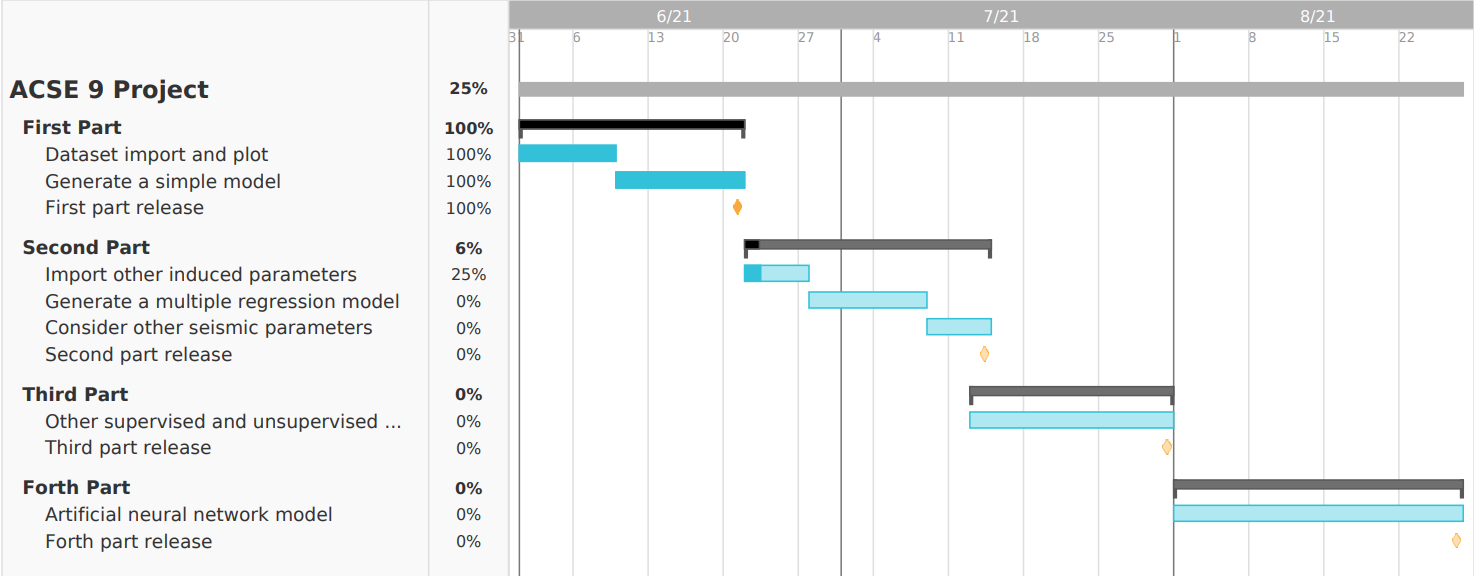
\includegraphics[width=1\textwidth]{gantt.png}
    \end{center}
    \caption{\label{fig:experiment} Gantt chart.}
\end{figure}

In this project, three potential parameters to investigate correlations with earthquake activity, which are injection volume, well depth and geological formation being injected into.
The parameters affected of earthquake activity considered are earthquake occurence, maximum earthquake magnitude and earthquake moment rate.
In the first part, dataset is successfully imported and plotted with geopandas. Then, as a starting point, injection vloume will be concentrated on to find the correlation with the earthquake occurence and produce a simple model. 
Here, some regression techniques such as linear or logistic regression will be used for the model generateing.
In the second part, other potential parameters (well depth and geological formation) will be introduced to consider together and a multiple regression model will be generated.
Besides, other earthquake activity parameters (maximum earthquake magnitude and earthquake moment rate) will be investigated correlations with induced potential parameters.
In the third part, a neural network model will be trained and generated with predictive capabilities.
In the final part, the project report will be focused on. 

% References
\bibliographystyle{agsm}
\bibliography{references.bib}  % BibTeX references are saved in references.bib

\end{document}          
